% =====================================================================
% soutenance.tex -- Modèle de diaporama de soutenance de PFE,
%                   Master TSI (M2), Aix-Marseille Université
%
% DURÉE DE L'EXPOSÉ
%   8 minutes pour un étudiant + 2 minutes par étudiant supplémentaire
%   (2 étudiants : 10 min, 3 : 12 min, 4 : 14 min), suivies des questions.
%   Repère : une diapositive par minute environ. Indiquez la taille du
%   groupe avec \nombreetudiants : le thème affiche un avertissement sur
%   la diapositive de titre si le diaporama est trop long (compiler deux
%   fois pour que le test soit à jour).
%
% CONTENU D'EXEMPLE
%   Les diapositives reprennent le projet d'exemple du modèle de rapport.
%   Remplacez le contenu par le vôtre en gardant la structure ; adaptez
%   ensuite votre discours au temps imparti.
%
% COMPILATION : pdflatex -> biber -> pdflatex -> pdflatex
%   (ou simplement : latexmk soutenance.tex ; Overleaf le fait seul).
% =====================================================================
\documentclass[aspectratio=169, 11pt]{beamer}
% Version imprimable, sans les apparitions successives :
% \documentclass[aspectratio=169, 11pt, handout]{beamer}

\usetheme{pfetsi}
% Avec une diapositive de transition au début de chaque section :
% \usetheme[intercalaires]{pfetsi}

\usepackage[french]{babel}
\frenchsetup{StandardItemizeEnv=true, StandardItemLabels=true}
\usepackage{bm}                 % vecteurs en gras : \bm{u}
\usepackage{booktabs}           % tableaux : \toprule, \midrule...
\usepackage{colortbl}           % ligne de tableau surlignée
\usepackage{siunitx}            % nombres et unités : \num{}, \qty{}{}
\sisetup{locale = FR}
\DeclareSIUnit{\pixel}{px}
\usepackage[tworuled, vlined, linesnumbered, french, onelanguage]{algorithm2e}
\usepackage{csquotes}
\usepackage[backend=biber, style=ieee, doi=false, isbn=false,
            eprint=false, url=false]{biblatex}
\addbibresource{references.bib}
\graphicspath{{figures/}}

% Vignette « image + légende » utilisée pour les résultats qualitatifs
\newcommand{\panneau}[2]{%
  \begin{minipage}[t]{0.19\textwidth}
    \centering
    \includegraphics[width=\linewidth]{#1}\\[1mm]
    \footnotesize #2
  \end{minipage}}

% Notes de l'orateur sur un second écran (décommentez pour les afficher) :
% \usepackage{pgfpages}
% \setbeameroption{show notes on second screen=right}

% --- Informations de la diapositive de titre --------------------------
\title{Estimation du flot optique par moindres carrés locaux}
\author{Alice DUPONT, Bastien MARTIN, Chloé BERNARD}
\institute{Aix-Marseille Université}
\date{Soutenance du 15 juin 2027}
\encadrants{Prénom NOM}
\nombreetudiants{3}                 % fixe la durée : 8 + 2 x (3 - 1) = 12 min
% \logoetablissement{figures/logo}  % logo facultatif (fichier à fournir)

\begin{document}

% Titre à gauche, plan à droite : le plan est généré à partir des
% \section. Gardez des titres de section courts.
\diapotitre

% =====================================================================
\section{Introduction}

% Une idée par diapositive. Le titre de la diapositive énonce cette idée.
\begin{frame}{Contexte et motivation}
  \begin{columns}[c]
    \begin{column}{0.48\textwidth}
      \begin{itemize}
        \item \alert{Flot optique} : déplacement apparent de chaque pixel
              entre deux images d'une séquence
        \item Applications : compression vidéo, suivi d'objets,
              stabilisation, robotique
        \item Besoins : précision \alert{sous-pixellique}, robustesse au
              bruit, rapidité
      \end{itemize}
    \end{column}
    \begin{column}{0.48\textwidth}
      \centering
      \begin{figure}
        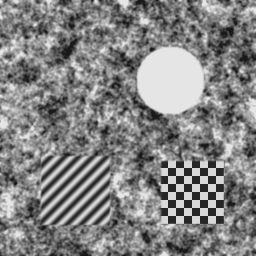
\includegraphics[width=0.48\linewidth]{s3_image}\hfill
        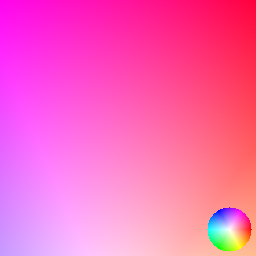
\includegraphics[width=0.48\linewidth]{s3_verite_terrain}
        \caption{Image et flot associé (la couleur code la direction,
          la saturation l'amplitude).}
      \end{figure}
    \end{column}
  \end{columns}
  \note[item]{Une phrase d'accroche : à quoi sert le flot optique ?}
  \note[item]{Montrer la roue des couleurs pour lire la figure.}
\end{frame}

% Apparition successive des points avec <+-> : utile pour guider
% l'auditoire, à utiliser avec modération.
\begin{frame}{Problématique et objectifs}
  \begin{itemize}[<+->]
    \item Conservation de la luminosité : \alert{une équation pour deux
          inconnues} $(u, v)$ en chaque pixel
    \item Méthodes existantes : précision limitée au pixel (blocs) ou
          coût élevé (régularisation globale)
  \end{itemize}
  \vspace{4mm}
  \uncover<3->{%
  \begin{block}{Objectif du projet}
    Une méthode \alert{locale}, sans apprentissage, avec une solution
    \alert{explicite} en chaque pixel et une précision sous-pixellique.
  \end{block}}
\end{frame}

% =====================================================================
\section{État de l'art}

% Colonnes : comparer des familles de méthodes côte à côte.
\begin{frame}{Méthodes existantes}
  \begin{columns}[T]
    \begin{column}{0.31\textwidth}
      \begin{block}{Blocs (BM)~\cite{jain1981}}
        \small
        \textcolor{tsiVert}{$+$} simple, robuste\\
        \textcolor{tsiAccent}{$-$} précision au pixel\\
        \textcolor{tsiAccent}{$-$} coût $\propto R^2$
      \end{block}
    \end{column}
    \begin{column}{0.31\textwidth}
      \begin{block}{Variationnelles~\cite{horn1981}}
        \small
        \textcolor{tsiVert}{$+$} champ dense et lisse\\
        \textcolor{tsiAccent}{$-$} coût de calcul\\
        \textcolor{tsiAccent}{$-$} lisse les contours
      \end{block}
    \end{column}
    \begin{column}{0.31\textwidth}
      \begin{block}{Apprentissage~\cite{dosovitskiy2015, teed2020}}
        \small
        \textcolor{tsiVert}{$+$} meilleure précision\\
        \textcolor{tsiAccent}{$-$} données, GPU\\
        \textcolor{tsiAccent}{$-$} peu interprétables
      \end{block}
    \end{column}
  \end{columns}
\end{frame}

% =====================================================================
\section{Méthodologie}

\begin{frame}{Formulation du problème}
  \begin{block}{Conservation de la luminosité}
    \[
      I_2(\bm{x} + \bm{u}) = I_1(\bm{x})
      \quad\xrightarrow{\text{Taylor}}\quad
      \nabla I^\top \bm{u} + I_t = 0
    \]
  \end{block}
  \vspace{2mm}
  \begin{itemize}
    \item $\nabla I = (I_x, I_y)^\top$ : gradient spatial ;
          $I_t = I_2 - I_1$ : dérivée temporelle
    \item Valable pour de petits déplacements
  \end{itemize}
  \vspace{2mm}
  \begin{alertblock}{Problème d'ouverture}
    Seule la composante de $\bm{u}$ parallèle au gradient est contrainte.
  \end{alertblock}
\end{frame}

% Équations dévoilées étape par étape avec \uncover<n->.
\begin{frame}{Moindres carrés locaux et critère de fiabilité}
  Hypothèse : $\bm{u}$ constant sur une fenêtre gaussienne $w$
  \[
    \hat{\bm{u}} = \arg\min_{\bm{u}} \sum_{\bm{y}} w(\bm{y} - \bm{x})
    \bigl( \nabla I(\bm{y})^\top \bm{u} + I_t(\bm{y}) \bigr)^2
  \]
  \uncover<2->{%
  Solution explicite : système $2 \times 2$
  \[
    \mathbf{T} \hat{\bm{u}} = -\bm{b}, \qquad
    \mathbf{T} = \sum w
    \begin{pmatrix} I_x^2 & I_x I_y \\ I_x I_y & I_y^2 \end{pmatrix},
    \qquad
    \bm{b} = \sum w \begin{pmatrix} I_x I_t \\ I_y I_t \end{pmatrix}
  \]}
  \uncover<3->{%
  \begin{exampleblock}{Critère de fiabilité}
    Estimation retenue seulement si $\lambda_{\min}(\mathbf{T}) > \tau$ :
    sinon zone homogène ou arête (problème d'ouverture).
  \end{exampleblock}}
\end{frame}

\begin{frame}{Extension pyramidale}
  \begin{columns}[c]
    \begin{column}{0.58\textwidth}
      \centering
      % =====================================================================
% schema_pyramide.tex -- Schéma-bloc dessiné avec TikZ
% Inclus dans soutenance.tex par % =====================================================================
% schema_pyramide.tex -- Schéma-bloc dessiné avec TikZ
% Inclus dans soutenance.tex par % =====================================================================
% schema_pyramide.tex -- Schéma-bloc dessiné avec TikZ
% Inclus dans soutenance.tex par \input{figures/schema_pyramide}.
% Un schéma TikZ utilise automatiquement les polices du document.
% =====================================================================
\begin{tikzpicture}[
    font=\footnotesize,
    >={Stealth[length=4pt]},
    image/.style={draw, fill=black!12, inner sep=0pt},
    bloc/.style={draw, rounded corners=2pt, fill=black!4, align=center,
                 inner sep=3pt, minimum height=8mm, text width=27mm},
    lien/.style={->, semithick},
  ]
  % Pyramides gaussiennes de I1 et I2 (niveau 2 = le plus grossier)
  \foreach \n/\c/\y in {2/4/0, 1/7/-15, 0/10/-31} {
    \node[image, minimum size=\c mm] at (0.8mm, \y mm - 0.8mm) {};
    \node[image, minimum size=\c mm] (p\n) at (0, \y mm) {};
  }
  \node[left=3mm of p2, align=right] {niveau 2\\ $64 \times 64$};
  \node[left=3mm of p1, align=right] {niveau 1\\ $128 \times 128$};
  \node[left=3mm of p0, align=right] {niveau 0\\ $256 \times 256$};
  \node[above=2mm of p2] {$I_1^{(\ell)},\, I_2^{(\ell)}$};

  % Estimation à chaque niveau
  \node[bloc] (b2) at (33mm, 0)      {Estimation MCL\\ initialisée à $\bm{0}$};
  \node[bloc] (b1) at (33mm, -15mm)  {Raffinement MCL\\ ($K$ itérations)};
  \node[bloc] (b0) at (33mm, -31mm)  {Raffinement MCL\\ ($K$ itérations)};
  \foreach \n in {2, 1, 0} {
    \draw[lien] (p\n.east) ++(0.8mm, 0) -- (b\n.west);
  }

  % Propagation du champ vers le niveau plus fin
  \draw[lien] (b2) -- node[right, align=left] {$\bm{u}^{(2)}$\\ $\uparrow 2,\ \times 2$} (b1);
  \draw[lien] (b1) -- node[right, align=left] {$\bm{u}^{(1)}$\\ $\uparrow 2,\ \times 2$} (b0);
  \draw[lien] (b0.east) -- ++(6mm, 0) node[right] {$\hat{\bm{u}}$};
\end{tikzpicture}
.
% Un schéma TikZ utilise automatiquement les polices du document.
% =====================================================================
\begin{tikzpicture}[
    font=\footnotesize,
    >={Stealth[length=4pt]},
    image/.style={draw, fill=black!12, inner sep=0pt},
    bloc/.style={draw, rounded corners=2pt, fill=black!4, align=center,
                 inner sep=3pt, minimum height=8mm, text width=27mm},
    lien/.style={->, semithick},
  ]
  % Pyramides gaussiennes de I1 et I2 (niveau 2 = le plus grossier)
  \foreach \n/\c/\y in {2/4/0, 1/7/-15, 0/10/-31} {
    \node[image, minimum size=\c mm] at (0.8mm, \y mm - 0.8mm) {};
    \node[image, minimum size=\c mm] (p\n) at (0, \y mm) {};
  }
  \node[left=3mm of p2, align=right] {niveau 2\\ $64 \times 64$};
  \node[left=3mm of p1, align=right] {niveau 1\\ $128 \times 128$};
  \node[left=3mm of p0, align=right] {niveau 0\\ $256 \times 256$};
  \node[above=2mm of p2] {$I_1^{(\ell)},\, I_2^{(\ell)}$};

  % Estimation à chaque niveau
  \node[bloc] (b2) at (33mm, 0)      {Estimation MCL\\ initialisée à $\bm{0}$};
  \node[bloc] (b1) at (33mm, -15mm)  {Raffinement MCL\\ ($K$ itérations)};
  \node[bloc] (b0) at (33mm, -31mm)  {Raffinement MCL\\ ($K$ itérations)};
  \foreach \n in {2, 1, 0} {
    \draw[lien] (p\n.east) ++(0.8mm, 0) -- (b\n.west);
  }

  % Propagation du champ vers le niveau plus fin
  \draw[lien] (b2) -- node[right, align=left] {$\bm{u}^{(2)}$\\ $\uparrow 2,\ \times 2$} (b1);
  \draw[lien] (b1) -- node[right, align=left] {$\bm{u}^{(1)}$\\ $\uparrow 2,\ \times 2$} (b0);
  \draw[lien] (b0.east) -- ++(6mm, 0) node[right] {$\hat{\bm{u}}$};
\end{tikzpicture}
.
% Un schéma TikZ utilise automatiquement les polices du document.
% =====================================================================
\begin{tikzpicture}[
    font=\footnotesize,
    >={Stealth[length=4pt]},
    image/.style={draw, fill=black!12, inner sep=0pt},
    bloc/.style={draw, rounded corners=2pt, fill=black!4, align=center,
                 inner sep=3pt, minimum height=8mm, text width=27mm},
    lien/.style={->, semithick},
  ]
  % Pyramides gaussiennes de I1 et I2 (niveau 2 = le plus grossier)
  \foreach \n/\c/\y in {2/4/0, 1/7/-15, 0/10/-31} {
    \node[image, minimum size=\c mm] at (0.8mm, \y mm - 0.8mm) {};
    \node[image, minimum size=\c mm] (p\n) at (0, \y mm) {};
  }
  \node[left=3mm of p2, align=right] {niveau 2\\ $64 \times 64$};
  \node[left=3mm of p1, align=right] {niveau 1\\ $128 \times 128$};
  \node[left=3mm of p0, align=right] {niveau 0\\ $256 \times 256$};
  \node[above=2mm of p2] {$I_1^{(\ell)},\, I_2^{(\ell)}$};

  % Estimation à chaque niveau
  \node[bloc] (b2) at (33mm, 0)      {Estimation MCL\\ initialisée à $\bm{0}$};
  \node[bloc] (b1) at (33mm, -15mm)  {Raffinement MCL\\ ($K$ itérations)};
  \node[bloc] (b0) at (33mm, -31mm)  {Raffinement MCL\\ ($K$ itérations)};
  \foreach \n in {2, 1, 0} {
    \draw[lien] (p\n.east) ++(0.8mm, 0) -- (b\n.west);
  }

  % Propagation du champ vers le niveau plus fin
  \draw[lien] (b2) -- node[right, align=left] {$\bm{u}^{(2)}$\\ $\uparrow 2,\ \times 2$} (b1);
  \draw[lien] (b1) -- node[right, align=left] {$\bm{u}^{(1)}$\\ $\uparrow 2,\ \times 2$} (b0);
  \draw[lien] (b0.east) -- ++(6mm, 0) node[right] {$\hat{\bm{u}}$};
\end{tikzpicture}

    \end{column}
    \begin{column}{0.4\textwidth}
      \begin{itemize}
        \item Grands déplacements divisés par $2^{L-1}$ au niveau
              le plus grossier
        \item Raffinement itératif à chaque niveau ($K$ itérations)
        \item Coût $\mathcal{O}(N K \sigma_w)$, indépendant de
              l'amplitude du mouvement
      \end{itemize}
    \end{column}
  \end{columns}
\end{frame}

% =====================================================================
\section{Expérimentations}

\begin{frame}{Données et protocole}
  \begin{columns}[c]
    \begin{column}{0.3\textwidth}
      \begin{figure}
        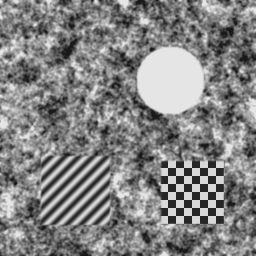
\includegraphics[width=\linewidth]{s3_image}
        \caption{Image synthétique : texture, zone homogène, rayures,
          damier.}
      \end{figure}
    \end{column}
    \begin{column}{0.66\textwidth}
      \small
      \begin{tabular}{@{}ll@{}}
        \toprule
        Séquence & Mouvement (vérité terrain connue) \\
        \midrule
        S1 & translation de $(\num{1.4}, \num{-0.7})$ pixel \\
        S2 & rotation de \ang{1} et zoom de \qty{1}{\percent} \\
        S3 & grand déplacement, jusqu'à \qty{11}{\pixel} \\
        \bottomrule
      \end{tabular}
      \vspace{4mm}
      \begin{itemize}
        \item Méthodes : \alert{MCL} (mono-échelle), \alert{MCL-P}
              (pyramidale), BM (blocs $9 \times 9$, $R = 10$)
        \item Métriques : EPE (pixels) et AAE (degrés)
      \end{itemize}
    \end{column}
  \end{columns}
\end{frame}

% Tableau : ne gardez que les colonnes utiles à votre message et
% surlignez le résultat à retenir.
\begin{frame}{Résultats quantitatifs}
  \centering
  \begin{tabular}{l *{3}{S[table-format=1.2] S[table-format=2.1]}
                  S[table-format=1.2]}
    \toprule
    & \multicolumn{2}{c}{S1} & \multicolumn{2}{c}{S2}
    & \multicolumn{2}{c}{S3} & {Temps} \\
    \cmidrule(lr){2-3} \cmidrule(lr){4-5} \cmidrule(lr){6-7}
    Méthode & {EPE} & {AAE} & {EPE} & {AAE} & {EPE} & {AAE} & {(\unit{\second})} \\
    \midrule
    BM    & 1.89 & 25.1 & 2.08 & 21.7 & 1.93 & 15.6 & 0.42 \\
    MCL   & 0.29 &  9.5 & 0.30 &  9.1 & 5.90 & 52.1 & 0.04 \\
    \rowcolor{tsiAccent!15}
    MCL-P & 0.13 &  2.9 & 0.10 &  2.4 & 0.28 &  0.9 & 0.07 \\
    \bottomrule
  \end{tabular}
  \vspace{5mm}
  \begin{itemize}
    \item MCL-P : erreur divisée par \alert{7 à 20} par rapport à BM,
          calcul environ \alert{6 fois} plus rapide
    \item La pyramide rattrape les grands déplacements (S3) ; l'avantage
          sur BM persiste en présence de bruit
  \end{itemize}
\end{frame}

% Figure dévoilée par étapes : \uncover<n->{...} réserve la place, ce qui
% évite que la mise en page ne « saute » d'une étape à l'autre.
\begin{frame}{Résultats qualitatifs (séquence S3)}
  \centering
  \panneau{s3_image}{Image $I_1$}\hfill
  \panneau{s3_verite_terrain}{Vérité terrain}\hfill
  \uncover<2->{\panneau{s3_bm}{BM}}\hfill
  \uncover<3->{\panneau{s3_mcl}{MCL}}\hfill
  \uncover<4->{\panneau{s3_mcl_p}{\alert{MCL-P}}}
  \vspace{5mm}
  \begin{itemize}
    \item<2-> BM : déplacements entiers, erreurs dans les zones homogènes
               et périodiques
    \item<3-> MCL : pas de mise à jour là où $\lambda_{\min}$ est faible
               (en blanc)
    \item<4-> MCL-P : proche de la vérité terrain ; erreurs résiduelles
               aux frontières des objets
  \end{itemize}
\end{frame}

% =====================================================================
\section{Conclusion}

\begin{frame}{Conclusion et perspectives}
  \begin{block}{À retenir}
    \begin{itemize}
      \item Estimation locale à solution explicite, avec un critère de
            fiabilité ($\lambda_{\min}$) et une extension pyramidale
      \item EPE de \num{0.10} à \qty{0.28}{\pixel}, contre environ
            \qty{2}{\pixel} pour BM, pour un calcul 6 fois plus rapide
    \end{itemize}
  \end{block}
  \vspace{2mm}
  \begin{exampleblock}{Perspectives}
    \begin{itemize}
      \item Suivi de points d'intérêt choisis là où $\lambda_{\min}$ est
            grand
      \item Modèle de mouvement affine par fenêtre
      \item Évaluation sur des séquences réelles (Middlebury)
    \end{itemize}
  \end{exampleblock}
\end{frame}

\diapoquestions

% =====================================================================
% Annexes : diapositives de secours pour répondre aux questions. Elles
% ne sont pas comptées dans le total ni dans la durée.
% =====================================================================
\annexes

\begin{frame}{Algorithme détaillé (MCL-P)}
  \begin{algorithm}[H]
    \DontPrintSemicolon
    \KwData{images $I_1$, $I_2$ ; paramètres $L$, $K$, $\sigma_w$, $\tau$}
    \KwResult{champ de déplacement $\hat{\bm{u}}$}
    Construire les pyramides $\{I_1^{(\ell)}\}$ et $\{I_2^{(\ell)}\}$\;
    $\hat{\bm{u}} \gets \bm{0}$ au niveau $L-1$\;
    \For{$\ell = L-1$ \KwTo $0$}{
      \lIf{$\ell < L-1$}{$\hat{\bm{u}} \gets 2 \times
        \text{suréchantillonner}(\hat{\bm{u}})$}
      Calculer $\nabla I_1^{(\ell)}$, $\mathbf{T}$ et $\lambda_{\min}$\;
      \For{$k = 1$ \KwTo $K$}{
        $I_t \gets I_2^{(\ell)}(\bm{x} + \hat{\bm{u}}) - I_1^{(\ell)}(\bm{x})$\;
        $\hat{\bm{u}} \gets \hat{\bm{u}} - \mathbf{T}^{-1} \bm{b}$
        là où $\lambda_{\min} > \tau$\;
      }
    }
  \end{algorithm}
\end{frame}

\begin{frame}{Complexité}
  Pour une image de $N$ pixels :
  \[
    C_{\text{MCL-P}} = \mathcal{O}(N K \sigma_w)
    \qquad\text{contre}\qquad
    C_{\text{BM}} = \mathcal{O}(N R^2)
  \]
  \begin{itemize}
    \item Filtrage gaussien séparable : $\mathcal{O}(\sigma_w)$ par pixel
    \item Pyramide : facteur $1 + 1/4 + 1/16 + \dots < 4/3$
    \item Paramètres : $\sigma_w = \num{2.5}$, $\tau = \num{e-4}$, $K = 5$,
          $L = 4$
  \end{itemize}
\end{frame}

% Références : seules les entrées citées apparaissent.
\begin{frame}[allowframebreaks]{Références}
  \footnotesize
  \printbibliography[heading=none]
\end{frame}

\end{document}
